\section{Detailed Design and Implementation}
\label{sec:design}


\subsection{Efficient Decoupled Speculative Rollout}
\label{sec:design-decouple}

\nospacestitle{Methodology. \,}
We adopt a two-step scheduling method to realize an efficient 
decoupled speculation:
(1) at the beginning of the rollout step,
we determine the optimal placement---how many workers are assigned to
drafting and verification, respectively---to minimize 
batch completion time.
During rollout, we (2) dynamically monitor the acceptance
rate of running requests to timely adjust their number of 
aggressively drafted tokens (with a draft window)
to minimize the impact of verification failures.

We choose to adjust only the draft window per request
but not the entire placement for the running batch during rollout for
three reasons. First, the optimal placement relies on
the modeling of system execution, but it becomes less
accurate due to the continuously reduced batch sizes caused by finished requests.
Second, the overhead of reconfiguring placement may outweigh the benefits.
Finally, since the batch sizes shrink quickly thanks to our decoupled execution
with optimal initial placement,
we no longer need to maximize computational efficiency,
and the fine-grained adjustment of the tail requests provided by (2)
enables sufficient speedups.

Below, we first describe how we control the wasted
tokens via \emph{draft window}, and then proceed to the two policies. 


\stitle{Drafting window ($w$) and relaxed draft--verification dependency. \,}
To control the waste due to mis-speculation,
we set a window similar to previous works~\cite{turbospec} such that:
once the drafter sends $w$ tokens to the
verifier,
it is only allowed to aggressively draft another $w$ tokens.
If the verifier has not finished verification,
the drafter stops waiting for the feedback from the verifier. 
In this way, the drafter wastes at most $2w - 1$ tokens under speculation failures,
as shown in {\fig{fig:decoupled-cases}}.



\begin{figure}[!t]
       \vspace{2mm}
        \begin{minipage}{1\linewidth}
        \centering    
        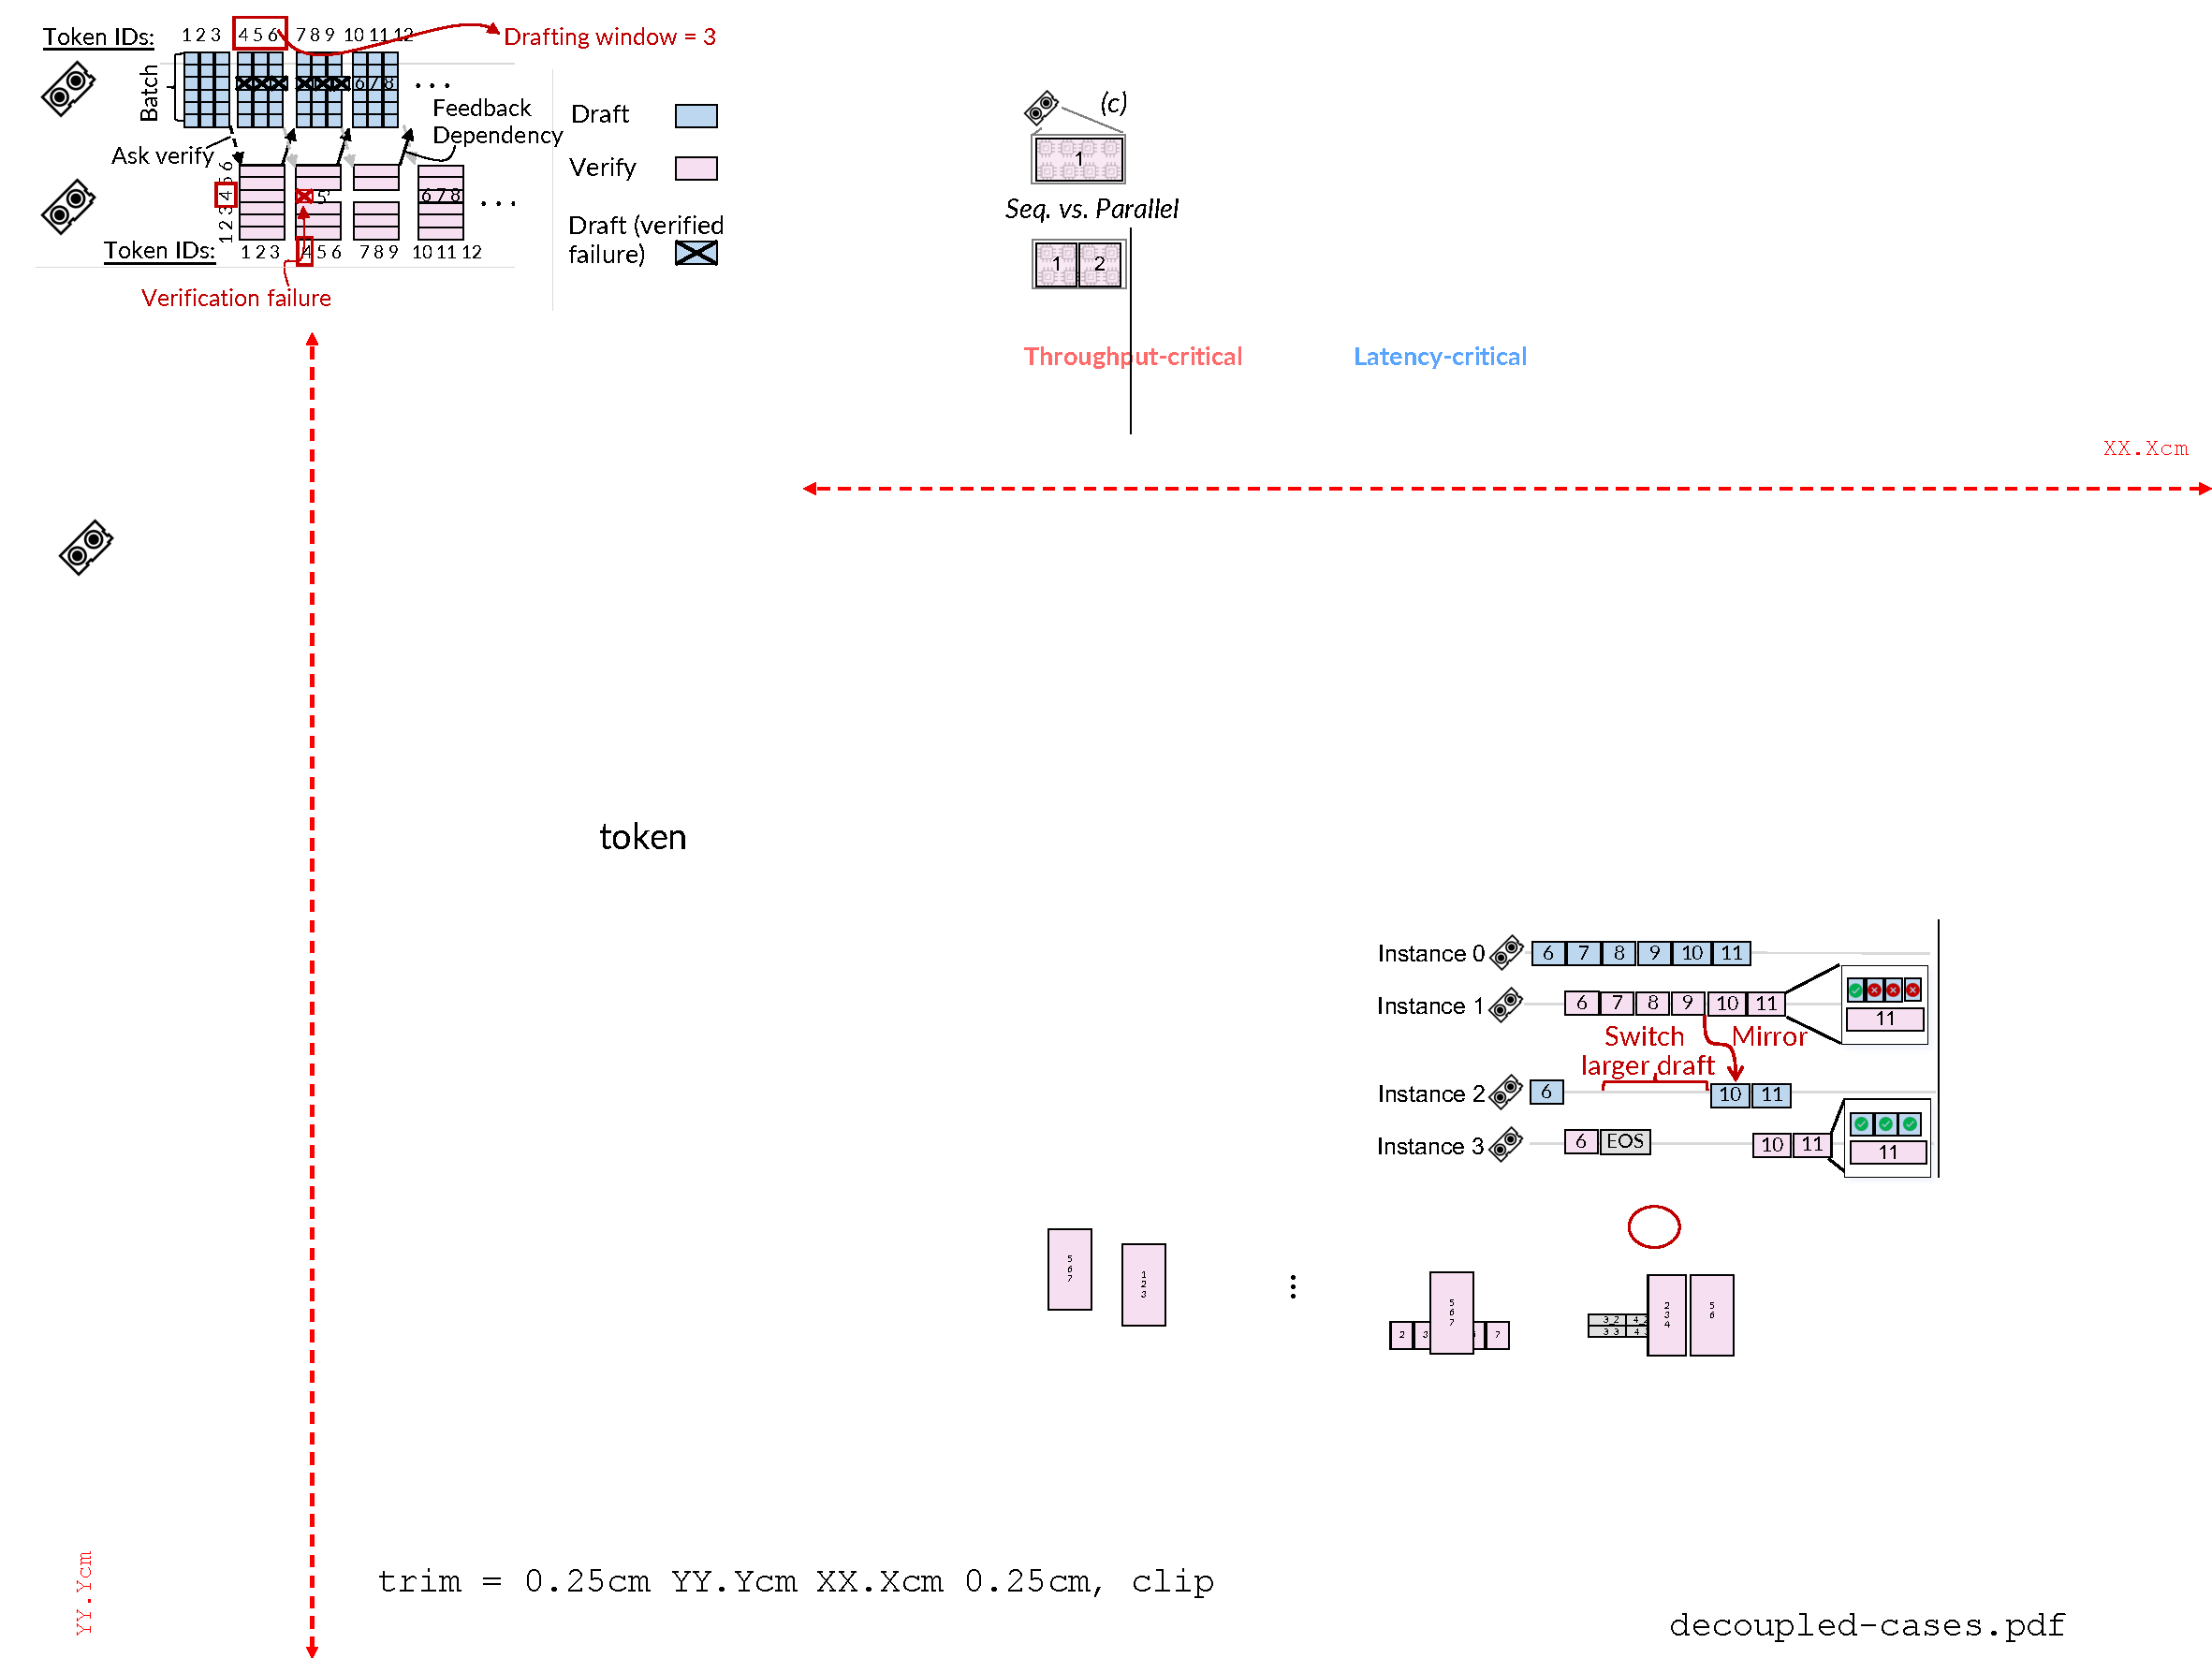
\includegraphics[width=0.95\linewidth, trim=0.25cm 24.0cm 26cm 0.25cm, clip]{figs/decoupled-cases.pdf} 
        \end{minipage} \\[0pt]
        \begin{minipage}{1\linewidth}
        \caption{\small{%
            An illustration of how relaxed decoupled execution 
            handle verification failure
            with a draft window of 3 tokens. 
        }}
        \label{fig:decoupled-cases}
        \end{minipage} \\[-15pt]
        \end{figure} 

\stitle{1. Decoupled speculation execution plan. \,}        
At the beginning of each rollout step,
given a draft method (described in \textsection{\ref{sec:design-bon}}),
the trained model, and the available GPUs,
our planner determines
an appropriate draft window for the entire batch, and
an efficient initial decoupled speculation plan by assigning
the drafter and verifier to different GPUs.
The plan only needs to be executed once during post-training
because for each step,
the initial batch size per worker remains the same,
and the acceptance length---average output length per verification 
are stable for mainstream drafters,
% (explained in \textsection{\ref{sec:design-bon}}),
as shown in \fig{fig:motiv-acc-len}. 
Our reported EAGLE acceptance length\footnote{\footnotesize{No prompt tuning was applied following TLT authors' instructions.}} is lower than that 
of TLT~\cite{tlt} because our rollout
temperature is set to 1.0 and we use a 
large-batch-tuned configuration---a common production setup in post-training~\cite{deepseek-r1,DBLP:journals/corr/abs-2402-03300,DBLP:journals/corr/abs-2507-20534}.

Finding the optimal execution plan requires solving a combination
problem of the parallel configurations of different drafters and verifiers,
as well as precisely modeling the performance of speculative decoding using the draft window.
To ease problem formulation, we follow prior works that
assume the developers have provided a set of possible GPU configurations for running a verifier ($\mathbb{G}$),
i.e., how one copy of model parameter is partitioned on a set of GPUs. 
For drafter, we assume it only uses one GPU as it is lightweight. 

Algorithm~\ref{alg:argmax-select} describes our algorithm, 
which is essentially an enumeration-based search with
decoupled-execution-aware pruning to accelerate the process.
{First, given a batch of requests to generate (\ie{$B$}),
we select a verification configuration (line 2),
and estimate its performance under decoupled execution ($\mathrm{TGS}_{\text{cur}}$)
for various numbers of draft GPUs (line 3) and
various draft window sizes (line {6}).
We continuously select execution plans and finally choose the one with the
minimal estimated generation time (line 8--10).}

To improve search time, we prune the enumeration space by
(1) using the observation that drafters need fewer GPUs than verifiers (line {3})
and (2) pruning arbitrarily large draft windows,
because it only increases the computation waste upon mis-speculation (line {5}).


\begin{figure}[!t]
       \vspace{2mm}
        \begin{minipage}{1\linewidth}
        \hspace{-1mm}
        \centering    
        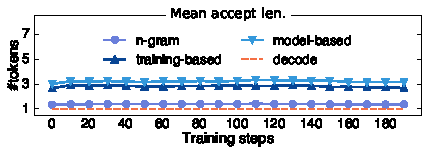
\includegraphics[width=\columnwidth]{data/motiv-acc-len.pdf} \\[3pt]    
        \end{minipage} \\[0pt]
        \begin{minipage}{1\linewidth}
        \caption{\small{%
        {
            Mean acceptance length profiled in a 200-step DAPO-32B-20K trace, covering 327\,K
            sequences. The training-based method uses \emph{frozen} EAGLE released 
            by TLT~\cite{tlt}.
        }}}
        \label{fig:motiv-acc-len}
        \end{minipage} \\[-10pt]
\end{figure}

\stitle{Modeling $\mathrm{TGS}$. \,}
A key aspect of the planning is to model the performance---\uline{t}oken 
\uline{g}eneration \uline{s}peed ($\mathrm{TGS}$)---for 
decoupled execution. 
We use a bottom-up approach that first models the execution time of drafter 
and verifier, then move on the modeling of 
the expectation of $\mathrm{TGS}$,
considering the impact of wasted tokens due to mis-speculation
under a selected draft window.

Given a batch of request $b$, the number of drafter workers $g_d$,
and a verifier with execution configuration $g_v$,
the draft ($D_{g_d}(\cdot)$) and verification ($V_{g_v,w}(\cdot)$) time can be approximated 
as an affine function with respective to the batch size ($b$):  \\[-10pt]
\begin{align*}
    {D_{g_d}(b)} &= b \cdot D_{g_d}' + \alpha_{g_d} \\
    {V_{g_v,w}(b)} &= b \cdot V_{g_v,w}' + \beta_{g_v,w}
\end{align*}
\noindent
where $D_{g_d}'$, $V_{g_v,w}'$, $\alpha_g$ and $\beta_{g_v,w}$ are 
hyperparameters that fitted through offline profiling,
similar to prior works~\cite{DBLP:conf/osdi/ZhuGZZZGX0KLWWK25,kunserve}. 

Therefore, the total generation time of $w$ tokens in our decoupled execution paradigm
can be modeled as: \\[-10pt]
\begin{align*}
    \mathrm{IL}_{g_d,g_v,w}(b) = \max \{wD_{g_d}(b), V_{g_v,w}(b)\}    
\end{align*}


Besides the execution time, we also need to consider the 
slowdown due to mis-speculation. 
Given a draft window $w$ and the probability of accepting one token $p$ for a batch of
requests, we follow prior works~\cite{DBLP:journals/corr/abs-2505-19645,turbospec} that
first model the probability of accepting $\alpha$ tokens
given $n$ tokens within a draft window,
then calculate the expected wasted tokens accordingly.
The difference is that we further consider the additional wasted tokens due to
aggressive speculation in decoupled execution. 
Specifically, within a draft window, 
the probability of accepting $a$ tokens 
given an estimated accept probability ($p$) is: \\[-10pt]:
\begin{align*}
    \mathrm{P}(a, w) &=
\begin{cases}
% 1-r^2, & a=1,\\[0.5em]
p^a (1 - p), & 0 \leq a \leq w - 1,\\[0.5em]
p^a, & a = w,
\end{cases} \\
    % \tau_{m,n} &= n r^{n} + \\ 
    % &\sum_{a=0}^{d-1} \frac{(a+2) p^a (1 - p) }{2} \\
    s.t.  &\quad a \in \mathbb{N}, n \in \mathbb{Z^+}
\end{align*}
\noindent
$p$ is profiled using the setup from previous steps 
and we found it is quite stable
for a relatively large batch of requests 
(see \fig{fig:motiv-acc-len}).

The expectation of the total generated tokens for drafting a draft window $w$ is: \\[-10pt]
\begin{equation*}
    \tau_w =
\overbrace{\sum_{a=0}^{w-1} p^{a}(1-p)
        \frac{a+1}{2}}^{\text{partial accept}}
+ \overbrace{w p^w}^{\text{full accept}}
\end{equation*}
\noindent 
which is a summation of the expected generated tokens when the token is accepted
at different positions.
    
% where we count the partial accepted iteration  and its 
% immediately-following draft window as a single iteration due to cascade rejection.
% For fully accepted iteration, 
% it can be treated as a unique random event ($a=w$).

Put it all together, the expectation of TGS is: \\[-5pt]
\begin{equation*}
    \mathrm{TGS}_{g_d,g_v,w}(b) = \frac{\tau_w}{\mathrm{IL}_{g_d,g_v,w}(b)}
\end{equation*}

\begin{algorithm}[t]
\caption{Decoupled execution plan generation algorithm at the start of the rollout. $\mathrm{TGS}_{g_d,g_v,w}(b)$,
$V_{g_v,w}(b)$ and $D_{g_d}(b)$ are descried in \textsection{\ref{sec:design-decouple}}. }
\label{alg:argmax-select}
\KwIn{%
Initial global batch size ${B}$, 
the number of GPUs in the cluster $G$,
a set of execution configurations for verification $\mathbb{G}$.
%    token generation speed function $\mathrm{TGS}_{g_d,g_v,w}(b)$, \\
%    verification time $V_{g_v,w}(b)$, draft time $D_{g_d}(b)$
}
\KwOut{%
    GPUs for drafting $g_{d}^*$, GPUs for verification $g_{v}^*$ and draft window $w^*$.
}

% $\mathrm{Votes} \gets \emptyset$\;

% \For{$b \gets 1$ \KwTo $B$}{
    $\mathrm{TGS}^* \gets 0$, $(g_{d}^*, g_{v}^*, w^*) \gets (0, 0, 0)$\;
    \ForEach{GPU number $g_v \in \mathbb{G}$}{
    \ForEach{GPU number $g_d \gets 1$ \KwTo $g_v$}{
        % $n_{\max} \gets \bigl\lceil V_n(b) \big/ D_g(b) \bigr\rceil$\;
        $b \gets \lceil \frac{(g_d + g_v)B}{G} \rceil$\;
        $w_{max} = \max\{\lceil \frac{V'_{g_v, w}}{D'_{g_d}} \rceil, \lceil \frac{\beta_{g_v, w}}{\alpha_{g_d}} \rceil\}$\;
        % $w_{\max} = \displaystyle\arg\min_{w} \ |V_{g_v, w}(b') - wD_{g_d}(b')|$\tcp*{Prune overlarge windows}
        \For{$w \gets 1$ \KwTo $w_{\max}$}{
            $\mathrm{TGS}_{\text{cur}} \gets \mathrm{TGS}_{g_d,g_v,w}(b)$\;
            
            \If{$\mathrm{TGS}_{\text{cur}} > \mathrm{TGS}^*$}{
                update $\mathrm{TGS}^*$ and $(g_{d}^*, g_{v}^*, w^*)$\;
                % $\mathrm{TGS}^* \gets \mathrm{TGS}_{\text{cur}}$\;
                % $(g_{d}^*, g_{v}^*, w^*) \gets (g_d, g_v, w)$\;
            }
        }
    }
    }
    % $\mathrm{Votes}[(g_{d}^*, g_{v}^*, w^*)] \gets \mathrm{Votes}[(g_{d}^*, g_{v}^*, w^*)] + 1$\;
% }
\Return{$(g_{d}^*, g_{v}^*, w^*)$}
\end{algorithm}


\begin{algorithm}[t]
\caption{Request-level Reconfiguration for Reducing mis-speculation overheads during the rollout. }
\label{alg:draft-adapt}

\KwIn{%
    pre-searched decoupled plan ($g_d^*, g_v^*, w^*$), \\
    the set of requests with lower acceptance rate than average $\mathbb{R}$.
}

\KwOut{%
    Per-request draft plan $\{(w_r, m_r)\}_{r \in \mathbb{R}}$,\\
    $w_r$ is request draft window, $m_r$ is a flag specifying coupled ($\textsc{c}$) or decoupled ($\textsc{d}$) speculation. 
}

% Initialize per-request tracking variables
% \ForEach{request $r \in \mathbb{R}$}{
%     $w_r, m_r \gets w^*, \textsc{decouple}$\;
% }


% Main speculative decoding loop with periodic adjustments
% \While{decoding system active}{
    % \If{$\text{niters} \geq T$}{
        % Greedy adjustment based on the last $T$ rounds
        \ForEach{request $r \in \mathbb{R}$}{
            $p \gets \text{ProfileProbability}(r)$\;
            $w_{\textsc{c}}, \text{tgs}_{\textsc{c}} \gets \displaystyle\arg\max_{w} \text{TGS}_{\textsc{c}, w}(p, b=1)$\;
            $w_{\textsc{d}}, \text{tgs}_{\textsc{d}} \gets \displaystyle\arg\max_{w} \text{TGS}_{g_d^*, g_v^*, w}(p, b=1)$\;
            $w_r, m_r \gets \text{SelectBetter}((w_{\textsc{c}},\text{tgs}_{\textsc{c}}), (w_{\textsc{d}},\text{tgs}_{\textsc{d}}))$
        }

        % $\text{niters} \gets 0$\;
    % }
    
    % Execute one speculative decoding round and accumulate statistics
    % \ForEach{request $r \in \mathbb{R}$}{
    %     $p \gets \text{GetPossibility}(r)$\;
    %     $a_r \gets a_r + \Delta{a}$\;
    % }
    % $\text{niters} \gets \text{niters} + 1$\;
% }

\Return{$\{(w_r, m_r): r \in \mathbb{R}\}$}
\end{algorithm}

\stitle{2. Dynamic request-level reconfiguration. \,}
During decoupled execution, we dynamically monitor each request's
acceptance rate to adjust its draft window accordingly. 
Algorithm~\ref{alg:draft-adapt} summarizes our reconfiguration algorithm,
which is called periodically during the rollout.

Upon invocation, the algorithm first examines the set of requests
{with lower acceptance rates than the average (line {1}),}
and reuses the performance model described above for decoupled execution 
and an extended modeling
of coupled execution
 ($\text{TGS}_{\textsc{c}, w}(\cdot)$, omitted due to space limitation,
 since its modeling logic is similar to decoupled modeling)
 to enumerate the best configuration.

Three aspects need to be noted regarding online reconfiguration.
First, we do not trigger reconfiguration too frequently
because (1) the acceptance rate may change sharply over a short period,
and (2) overly frequent reconfiguration may introduce performance instability.
Currently, we reconfigure the system every 1000 decoding iterations.
Second, we execute requests with different window sizes concurrently
to maximize GPU utilization.
To achieve efficient co-execution, we schedule kernels with different
draft windows into a fused CUDA graph~\cite{vllm-code,turbospec}.
Finally, switching between coupled and decoupled execution is straightforward,
as we only need to pause the aggressive draft of the switched request.

\subsection{Effective Fastest-of-N (FoN) Speculative Rollout}
\label{sec:design-bon}


\noindent
This section describes how we select draft methods for the rollout.
The goal is to select the method with the highest speedup.
The challenge lies in balancing the draft efficiency and the acceptance rate,
given that the acceptance rate is unknown prior to execution for a given request.

To tackle this challenge, we leverage the fact that
it is possible to estimate the speedup of different draft methods
parameterized by the acceptance rate
via offline profiling.
With this information, selecting draft methods greedily
using the average acceptance rate of a batch request
is possible at the beginning of the rollout,
and we can further improve the selection
based on the runtime-collected acceptance rate.

\begin{figure}[!t]
    %    \vspace{2mm}
        \begin{minipage}{1\linewidth}
        \hspace{-1mm}
        \centering    
        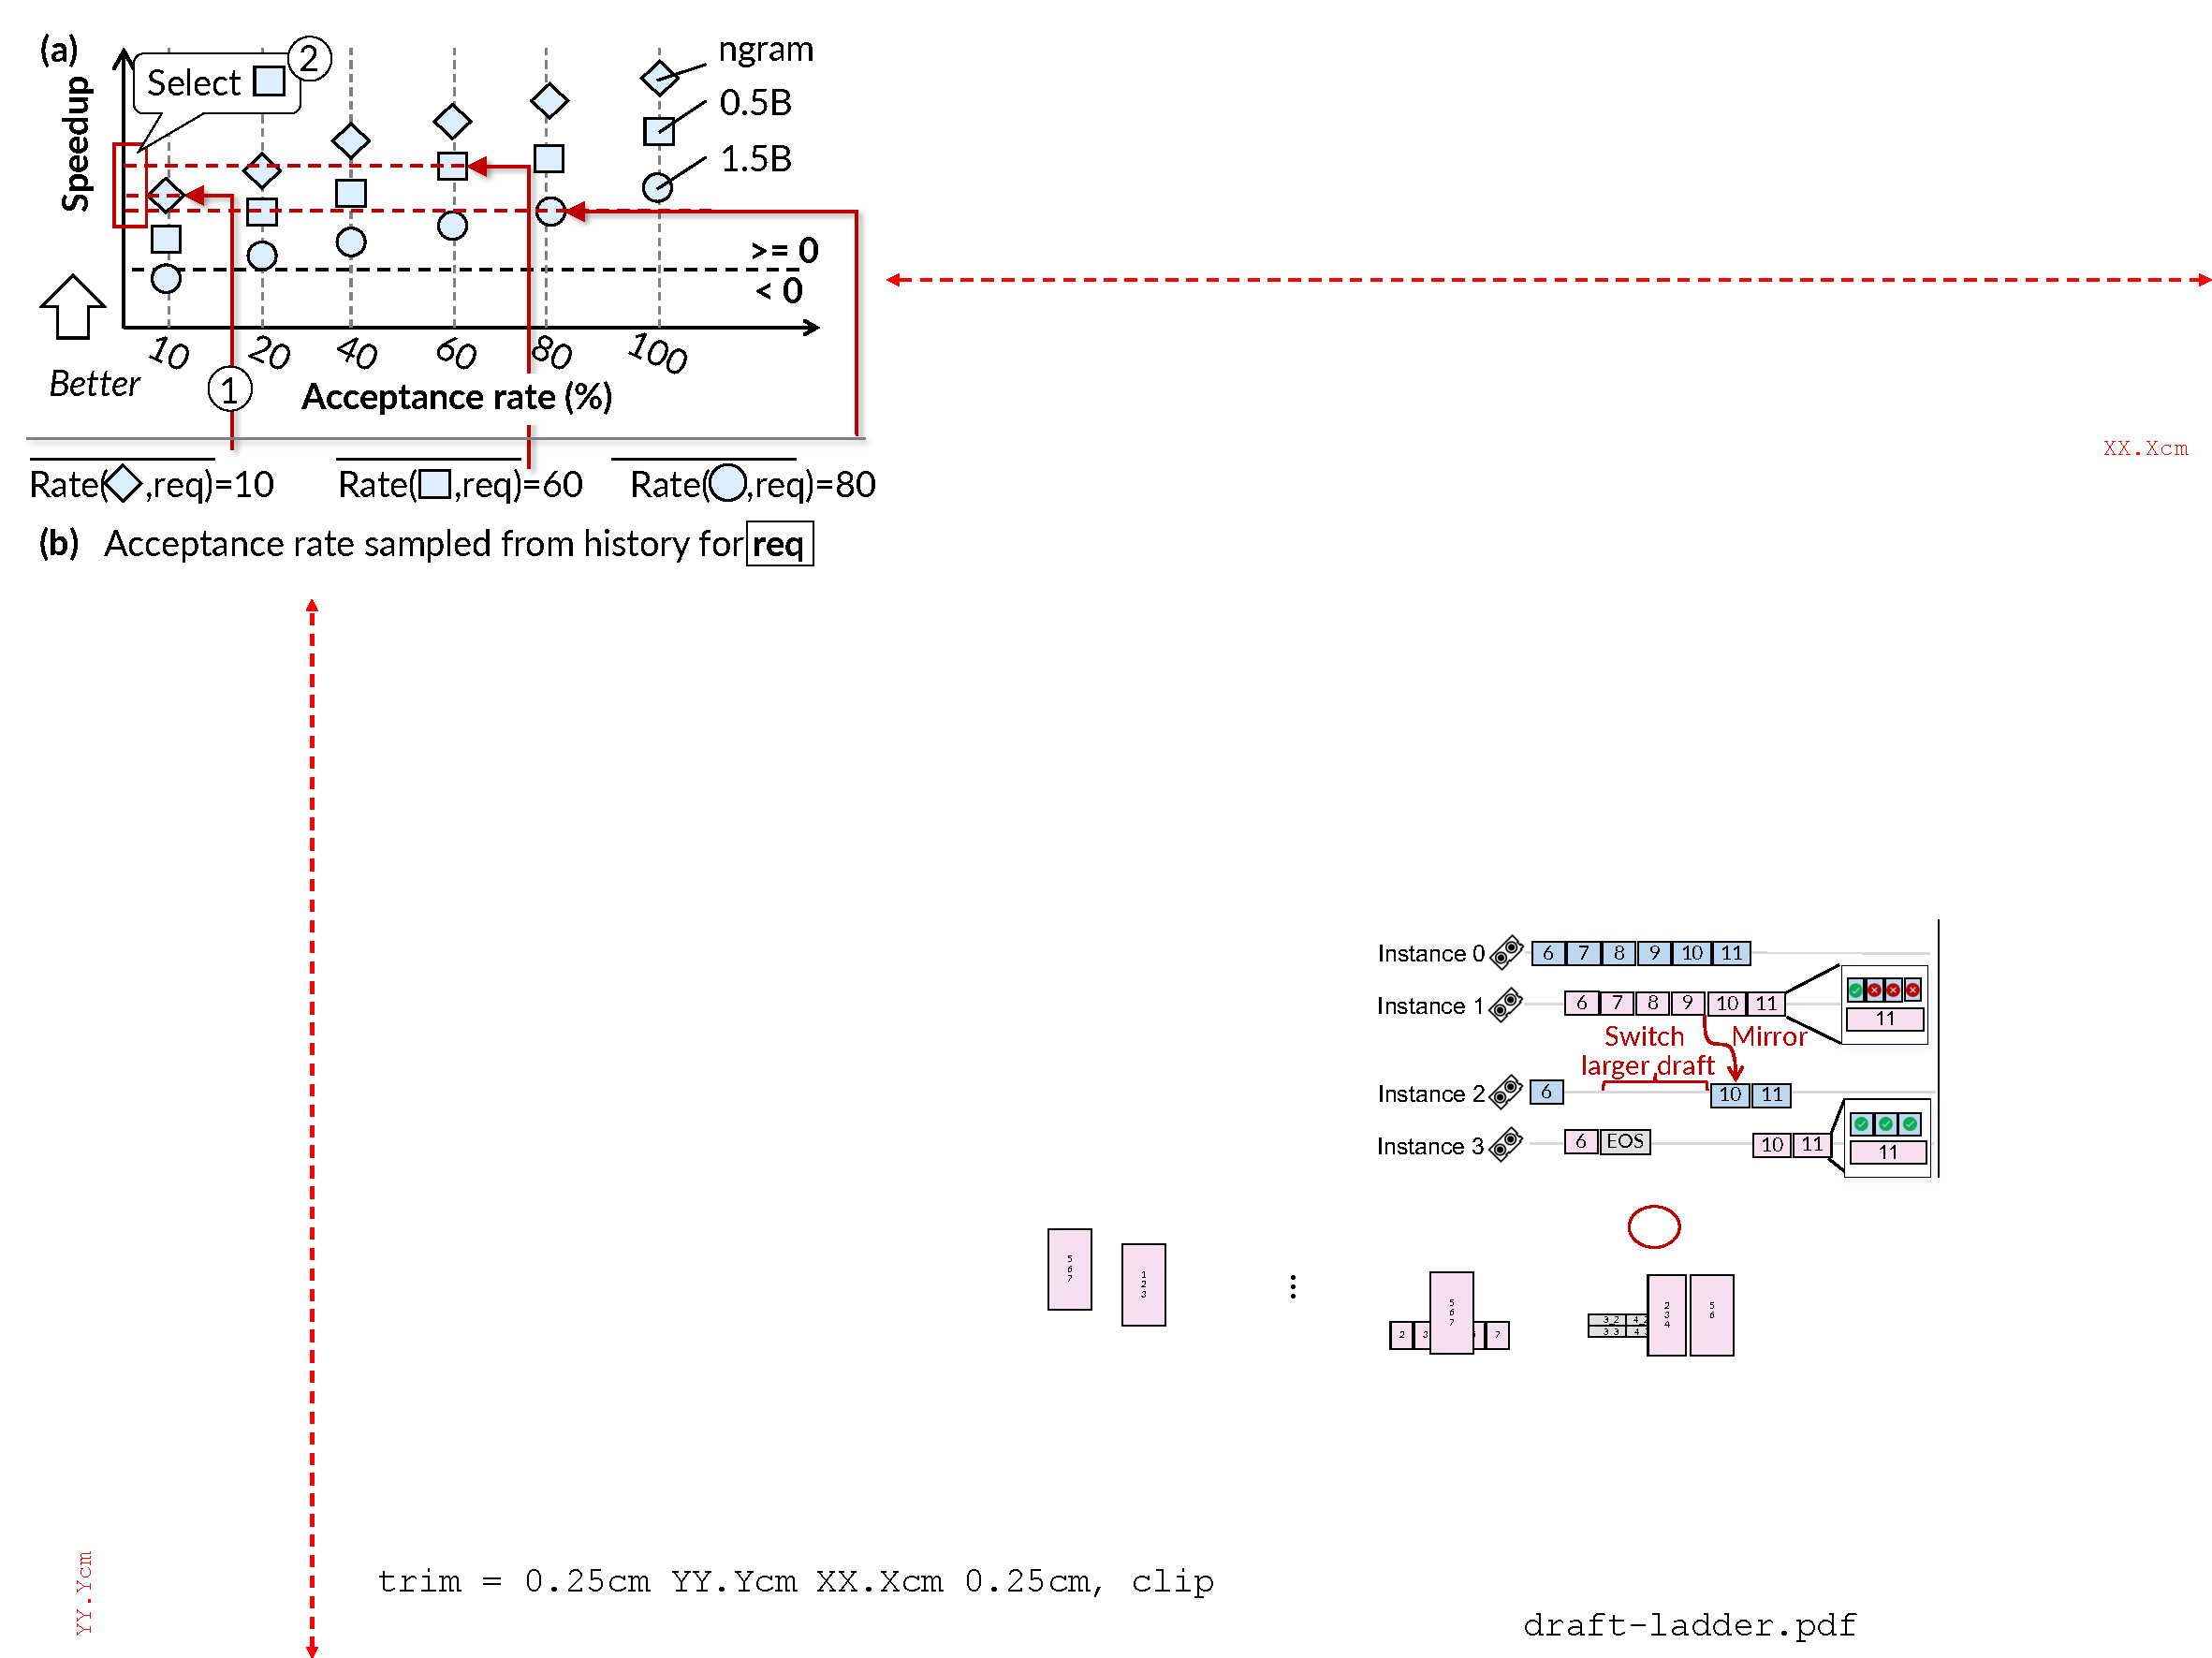
\includegraphics[width=0.85\columnwidth,trim=0.25cm 19.75cm 24cm 0.25cm, clip]{figs/draft-ladder.pdf} \\[3pt]
        \end{minipage} \\[10pt]
        \begin{minipage}{1\linewidth}
        \caption{\small{%
        {
            (a) Our draft ladder provides hints to the speedup of different draft methods and 
            (b) our ranking (\ding{192}) and selection (\ding{193}) mechanism for choosing
            a draft method. 
        }}}
        \label{fig:draft-ladder}
        \end{minipage} \\[-0pt]
\end{figure}

\stitle{Draft ladder. \,}
A draft ladder provides information on the speedup of different draft methods
given a fixed acceptance rate,
as shown in {\fig{fig:draft-ladder} (a)}.
It can be efficiently constructed via offline profiling
without using the trained model because
(1) the execution of the drafter is irrelevant to the training model and
(2) the speedup can be simulated by randomly accepting tokens according 
to a given acceptance rate.
Thus, our offline profiler directly run the draft methods
with simulated acceptance rate to build the ladder. 

Our current ladder considers popular draft methods, 
including model-based~\cite{spd,specinfer} and n-gram-based~\cite{pld,lookahead,DBLP:conf/acl/HuWZZLCZ25}. 
{For model-based draft, we use a checkpoint from the same series as the large model, 
released jointly before the post-training pipeline.
The practice is similar to previous inference works~\cite{spd,specinfer},
but we cannot use the thinking version draft models as they are typically
distilled after the large thinking model is ready~\cite{deepseek-r1,qwen3}.}
{We have also considered more draft methods,
including training-based drafters
such as the EAGLE family~\cite{eagle,eagle-2,eagle-3}.}
{We do not include MTP~\cite{DBLP:journals/corr/abs-2412-19437} as it is not 
integrated by our evaluated models.}
Nevertheless, we should emphasize that our design
is orthogonal to the draft methods,
and integrating more draft methods is likely to
make {\sys} faster if they can further improve speculation speedup.

\stitle{Draft method selection at the beginning of the rollout. \,}
Initially, we select \emph{one} draft method for
the entire batch based on the historically profiled acceptance rate.
{The profiling only needs to be done once, 
as the profiled results are stable across different steps 
(see \fig{fig:motiv-acc-len}).}
We cannot select multiple methods because each drafter requires 
similar amount of verification, 
and we have insufficient GPU computational power
during the initial phase.

{\fig{fig:draft-ladder} (b)} illustrates the selection process:
For three exemplified draft methods---n-gram, drafting with a 0.5B
and 1.5B model,
we first query the profiled acceptance rate of these methods,
and use these rates as the estimated acceptance rate of the batch.
Based on the rate, we can estimate the speedup of each draft method (\ding{192})
and then select the fastest one among them (\ding{193}).

\begin{algorithm}[t]
\caption{Greedy Fastest-of-N assignments. 
$b_{max}$ is the maximal verification batch size. 
}
\label{alg:bon-sched}

\KwIn{%
    the active requests set $\mathbb{R}$,  
    the candidate draft methods set $\mathbb{D}$.
    $\mathbb{W}_d$ is the set of workers responsible for draft method $d$,
    and $\mathbb{W}$ the whole set of free rollout workers.
}

\KwOut{%
    added drafters and the involved requests $\mathcal{M} = \{(r,d):w\}_{r \in \mathbb{R}, d \in \mathbb{D}, w \in \mathbb{W}}$.
}
% \ForEach{worker $w \in \mathbb{W}$}{
%     draft method $d\gets \displaystyle\arg\min_{d} \ |\mathbb{W}_{d}|$\;
%     $\mathbb{W}_{d} \gets \mathbb{W}_{d} \cup \{w\}$\;
% }

$\mathcal{R} \gets$ sort $\mathbb{R}$ by \text{GetAcceptRate}(r) ascending\;
$\mathcal{D} \gets$ sort $\mathbb{D}$ by \text{GetLadderRank}(d) ascending\;
\ForEach{request $r\in\mathcal{R}$}{
\ForEach{draft method $d\in\mathcal{D}$}{
    \If{$\mathcal{M}(r,d)$ is None}{
            $w \gets \text{GetMinLoadWorker}(\mathbb{W}_d, b_{max})$\;
            \If{$w$ is not None}{
                $\mathcal{M}(r,d) \gets w$\;
                $\text{load}(w)\mathrel{+}=1$\;
            }
    }
}
}

\Return{$\mathcal{M}$}
\end{algorithm}

%\stitle{Priority-based Fastest-of-N scheduling. \,}
\stitle{Greedy Fastest-of-N assignments. \,}
To cope with the sub-optimal initial selection for tailed requests,
we greedily deploy more draft methods as soon as
GPUs of both drafter and verifier become available upon batch completion.
\alg{alg:bon-sched} shows our algorithm for assigning
more drafters (and their corresponding verifier) when there are available workers.
The routine is iteratively called once there are free workers.


The algorithm assigns drafters to requests in an order sorted
by the reverse of their acceptance rate (lines 1)
as these requests have little speedup with speculative decoding.
For each request, we add a drafter with the highest
speedup according to the draft ladder described before 
if it has not been assigned yet (line 2 and 5).
We greedily assign as many drafters as possible to the request
until there are no available workers or pending requests (lines 3--9).
If the assignments for a request are completed,
we proceed to the next request.


Here we adopt a draft-first design that assigns as many draft methods to one request as possible before moving on to the next one.
The rationale is that the request with the lowest acceptance rate is likely to suffer from suboptimal drafting,
so the draft-first strategy can naturally select the optimal draft method for it (given a sufficient number of free workers).
In case of an insufficient number of free workers, we prioritize the draft method with a higher rank in our draft ladder.


\stitle{{Discussion for evolvable draft methods.} \,}
Our ladder assumes that the draft models are frozen during the post-training, 
because we found that the acceptance rate of draft methods remains stable 
across steps (even with long gap), see {\fig{fig:motiv-acc-len}}. 
%Although the alignment between draft and trained model shifts as training progresses, 
%the mean acceptance length remains stable over hundreds of steps (\TODO{see xx}).
% We conjecture that it is because even though the capability gap between the trained
% model and the drafter becomes larger during the training process,
% there are still many trivial tokens that can be drafted.
%We conjecture that, even as the capability gap grows, 
We suspect this is because even as the trained model becomes smarter,
many trivial tokens can still be drafted as long as the trained model corrects
the incorrect tokens timely. 
{Note that recent draft training optimizations~\cite{tlt} is orthogonal 
to our design as they can also be applied to our small models.}
Further, integrating such evolving would require
intrusive modifications to both the rollout and training engines.
Therefore, we don't include them in our implementation. 
%we do not include the design
%due to its additional cost of GPU hours and limited improvement 
%We should also mention that {\sys} is compatible with online draft evolving
%because our decoupled and Fastest-of-N designs has no assumption on the chosen draft methods.

\subsection{Efficient System Runtime for {\sys}}
\label{sec:design-mechanisms}

\noindent 
{\sys} only optimizes the rollout phase and makes no intrusive modifications
to the training engine, in contrast to~\cite{rlhfuse,rollpacker}.
The runtime extension is also lightweight:
supporting decoupled execution only requires message passing
between the drafter and the verifier,
and we further incorporate two primitives to support Fastest-of-N speculation:


% \vspace{0.1ex}
\stitle{Model scale. \,}
The primitive deploys a serving instance—--either a drafter or a verifier—to a specific worker.
This is similar to model autoscaling in existing serving engines~\cite{DBLP:conf/osdi/FuXHBUPM24,DBLP:conf/sosp/Xiang0QYZYZL0025,DBLP:conf/sosp/WeiHSH0H0025,DBLP:conf/asplos/ZengXGCL25,DBLP:conf/osdi/ZhangWLWS0025} 
and we adopted all their designs, 
including pre-pinning serving engines on workers~\cite{DBLP:conf/sosp/Xiang0QYZYZL0025},
pre-materializing CUDA graphs with GPU execution context pools~\cite{DBLP:conf/asplos/ZengXGCL25,DBLP:conf/sosp/WeiHSH0H0025}
and transfer model weights via fast networking between GPUs~\cite{DBLP:conf/osdi/ZhangWLWS0025}. 
To further eliminate the overhead of loading large trained model weights to GPUs
especially in case of deploying a new verifier, 
we observed that verifiers are deployed only to freed drafters and the 
drafter GPUs have low GPU memory usage due to the small size of draft models. 
Thus, we further pin the trained models to drafters to enable a zero-cost verifier deployment. 


\stitle{KVCache scale. \,}
Besides the model, when scaling a new drafter's corresponding verifier,
the new verifier requires a copy of the KVCache---the intermediate results
of the LLM computation---to accelerate computation.
A challenge is that during the later stage of rollout,
the KVCache may become large since its size is proportional to the model size and the number of
generated tokens.
To this end, we can leverage the classic KVCache recovery method,
which transfers the tail KVCache through the network
and recomputes it from the beginning~\cite{DBLP:journals/corr/abs-2410-03065}
to accelerate the KVCache scaling.

